\clearpage
\VerdierPhysicalPageAnchor{0237}%
\begingroup\small\setlength{\parskip}{0pt}\setlength{\emergencystretch}{1.5em}
\setlength{\abovedisplayskip}{4pt plus 2pt minus 2pt}%
\setlength{\belowdisplayskip}{4pt plus 2pt minus 2pt}%

\VerdierSemanticAnchor{ch4d-4-3-2}
\noindent\textbf{命题 4.3.2.}\quad
\textit{设 $X$ 是 $\operatorname{comp}(\mathcal A)$ 的对象，
$\bigl(X(p,q),\delta(p,q,r)\bigr)$ 是与 $X$ 相联系的第二谱对象，并设
$H\colon D(\mathcal A)\longrightarrow\mathcal A$ 是典范上同调函子。}

\VerdierSemanticAnchor{ch4d-4-3-2-a}
\noindent\textit{a) 对每个整数 $r<p$ 或 $r\geq q$，有
$H^r\bigl(X(p,q)\bigr)=0$。}

\VerdierSemanticAnchor{ch4d-4-3-2-b}
\noindent\textit{b) 设 $r$ 是整数。对
$\mathcal{F}\ell_1(\widetilde{\mathbb Z})$ 中满足 $p\leq r<q$ 的每个元素
$(p,q)$，存在唯一同构}
\[
i_{p,q}^r(X)\colon H^r(X)\xrightarrow{\sim}H^r\bigl(X(p,q)\bigr)
\]
\noindent\textit{使得 $i_{-\infty,+\infty}^r(X)$ 是恒等态射，并且对每一对
$(p,q)$ 与 $(p',q')$，若 $p\leq p'$、$q\leq q'$、$p\leq r<q$ 且
$p'\leq r<q'$，下图交换：}

\VerdierSemanticAnchor{ch4d-4-3-2-b-diagram}
\begin{center}
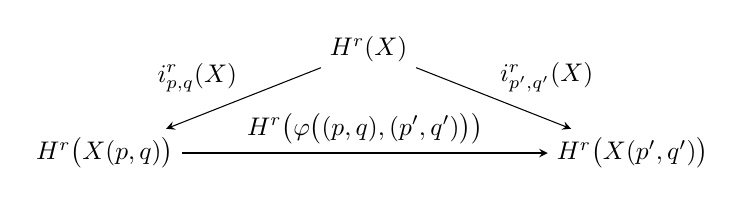
\begin{tikzpicture}[>=stealth,line width=.38pt,x=2.35cm,y=1.15cm,
  scale=.92,transform shape]
  \node (HX)  at (1.55,1.25) {$H^r(X)$};
  \node (Hpq) at (0,0) {$H^r\bigl(X(p,q)\bigr)$};
  \node (Hpp) at (3.10,0) {$H^r\bigl(X(p',q')\bigr)$};
  \draw[->] (HX) -- node[above left=-1pt] {$i_{p,q}^r(X)$} (Hpq);
  \draw[->] (HX) -- node[above right=-1pt] {$i_{p',q'}^r(X)$} (Hpp);
  \draw[->] (Hpq) -- node[above]
    {$H^r\!\left(\varphi\bigl((p,q),(p',q')\bigr)\right)$} (Hpp);
\end{tikzpicture}
\end{center}

\VerdierSemanticAnchor{ch4d-4-3-2-c}
\noindent\textit{c) 设 $m\colon X\longrightarrow Y$ 是
$\operatorname{comp}(\mathcal A)$ 中的态射，并设}
\[
m(p,q)\colon X(p,q)\longrightarrow Y(p,q)
\]
\noindent\textit{是相应的两个关联第二谱对象之间的态射。对
$\mathcal{F}\ell_1(\widetilde{\mathbb Z})$ 的每个元素 $(p,q)$ 以及满足
$p\leq r<q$ 的每个整数 $r$，下图交换：}

\VerdierSemanticAnchor{ch4d-4-3-2-c-diagram}
\begin{center}
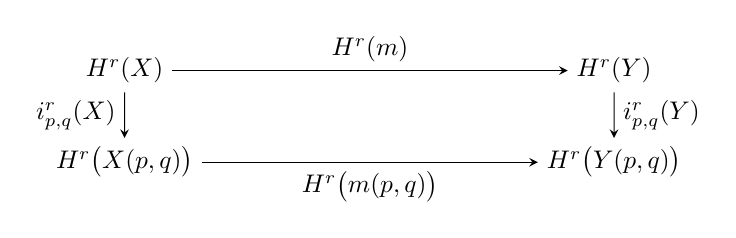
\begin{tikzpicture}[>=stealth,line width=.38pt,x=2.55cm,y=1.10cm,
  scale=.92,transform shape]
  \node (HX)  at (0,1.15) {$H^r(X)$};
  \node (HY)  at (2.65,1.15) {$H^r(Y)$};
  \node (Hpq) at (0,0) {$H^r\bigl(X(p,q)\bigr)$};
  \node (HpY) at (2.65,0) {$H^r\bigl(Y(p,q)\bigr)$};
  \draw[->] (HX) -- node[above] {$H^r(m)$} (HY);
  \draw[->] (Hpq) -- node[below] {$H^r\bigl(m(p,q)\bigr)$} (HpY);
  \draw[->] (HX) -- node[left] {$i_{p,q}^r(X)$} (Hpq);
  \draw[->] (HY) -- node[right] {$i_{p,q}^r(Y)$} (HpY);
\end{tikzpicture}
\end{center}

\noindent 此命题由定义立即得出。

\VerdierSemanticAnchor{ch4d-4-3-3}
\medskip\noindent\textbf{推论 4.3.3.}\quad
\textit{第二典范谱对象函子 (4.3.1) 唯一地通过典范函子}
\[
\operatorname{comp}(\mathcal A)\longrightarrow D(\mathcal A).
\]
\noindent\textit{分解。}

\VerdierSemanticAnchor{ch4d-4-3-3-proof}
事实上，由 (4.3.2)，此函子把拟同构 $m\colon X\longrightarrow Y$ 变为
谱对象的同构。因此，该推论由 (1.3.5) 得出。
\endgroup
